%%%%%%%%%%%%%%%%%%%%%%%%%%%%%%%%%%%%%%%%%
% Beamer Presentation
% LaTeX Template
% Version 1.0 (10/11/12)
%
% This template has been downloaded from:
% http://www.LaTeXTemplates.com
%
% License:
% CC BY-NC-SA 3.0 (http://creativecommons.org/licenses/by-nc-sa/3.0/)
%
%%%%%%%%%%%%%%%%%%%%%%%%%%%%%%%%%%%%%%%%%

%----------------------------------------------------------------------------------------
%	PACKAGES AND THEMES
%----------------------------------------------------------------------------------------

\documentclass[usenames,dvipsnames,table]{beamer}

\mode<presentation> {

\usetheme{Madrid}
%\setbeamertemplate{footline} % To remove the footer line in all slides uncomment this line
%\setbeamertemplate{footline}[page number] % To replace the footer line in all slides with a simple slide count uncomment this line
\setbeamertemplate{navigation symbols}{} % To remove the navigation symbols from the bottom of all slides uncomment this line
}

\usepackage{amsmath}
\usepackage{graphicx} % Allows including images
\usepackage{booktabs} % Allows the use of \toprule, \midrule and \bottomrule in tables
\usepackage{listings}
\usepackage{xcolor}
\usepackage{xfrac}
% \usepackage{enumitem}

\usefonttheme[onlymath]{serif}

%----------------------------------------------------------------------------------------
%	TITLE PAGE
%----------------------------------------------------------------------------------------

\title[ABDA Ch 17]{Applied Bayesian Data Analysis --- Chapter 17}

\author{Kim Albertsson} % Your name
\institute[LTU and CERN]
{
CERN and Luleå University of Technology \\
\medskip
\textit{kim.albertsson@ltu.se}
}
\date{\today}

\newcommand{\cgy}{\cellcolor{gray!25}}
\newcommand{\cgr}{\cellcolor{green!25}}
\newcommand{\cye}{\cellcolor{orange!25}}
\newcommand{\ccb}{\cellcolor{Cerulean!25}}

\begin{document}

\begin{frame}
\titlepage % Print the title page as the first slide
\end{frame}

% \begin{frame}
% \frametitle{}
% \begin{itemize}
% \item
% \end{itemize}
% \end{frame}

%----------------------------------------------------------------------------------------
%	PRESENTATION SLIDES
%----------------------------------------------------------------------------------------
\section{Chapter 17}
\begin{frame}
\begin{center}
{\huge{Chapter 17}}
\Large
\\\vspace{2em}
Metric predicted Variable with One Metric Predictor\\
\vspace{1em}
\textcolor{gray}{A.k.a. Univariate Regression}
\vspace{5em}
\end{center}
\end{frame}


\begin{frame}
\frametitle{Recap of where we are}

\textbf{So far:} Modelled a central tendency with added noise.
\begin{align*}
y = \beta_0 + \varepsilon
  \implies y &\sim \mathcal{N}(\beta_0 + \mu_\varepsilon, \sigma_\varepsilon) \\
             &\sim \mathcal{N}(\mu, \sigma)
\end{align*}

\textbf{In hierarchical models:} Noise was \emph{structured}, i.e. we changed the form of $\mu_\varepsilon$ and $\sigma_\varepsilon$.

\vspace{1em}
\textbf{Now:} Expand structure in central tendency estimation
\begin{align*}
y  = \beta_0 + \beta_1 x + \varepsilon
  \implies y &\sim \mathcal{N}(\beta_0 + \beta_1 x + \mu_\varepsilon, \sigma_\varepsilon)\\
             &\sim \mathcal{N}(\mu=c_0 + \beta_1 x, \sigma)
\end{align*}

\textbf{Note:} We can use regression on any parameter e.g. $\sigma$, however, the model $y = \beta_0 + \beta_1 x + \varepsilon$ is a very useful one, hence we focus on this first.
\end{frame}

\begin{frame}
\frametitle{Recap of where we are (in pictures!)}
\begin{columns}
\column{.5\textwidth}
The first kind of model we considered was:
\begin{align*}
\textrm{model: } y      &\sim \operatorname{pdf}(\theta) \\
\textrm{prior: } \theta &\sim \operatorname{pdf}(\varphi) \\
                   \varphi &= \varPhi
\end{align*}
\column{.5\textwidth}
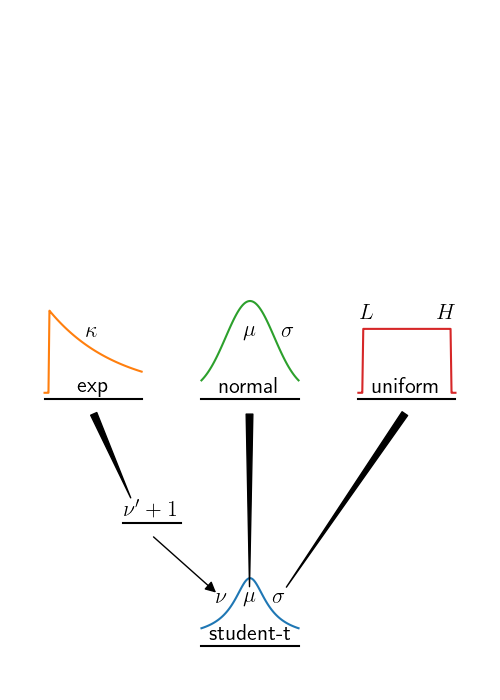
\includegraphics[width=\textwidth]{img/progress-base}
\end{columns}
\end{frame}

\begin{frame}
\frametitle{Recap of where we are (in pictures!)}
\begin{columns}
\column{.5\textwidth}
We then considered hierarchical models, these provide \emph{structured noise}:
\begin{align*}
\textrm{model: } y      &\sim \operatorname{pdf}(\theta) \\
\textrm{prior: } \theta &\sim \operatorname{pdf}(\varphi) \\
                   \varphi &\sim \operatorname{pdf}(\lambda) \\
                   \lambda &= \Lambda
\end{align*}
\column{.5\textwidth}
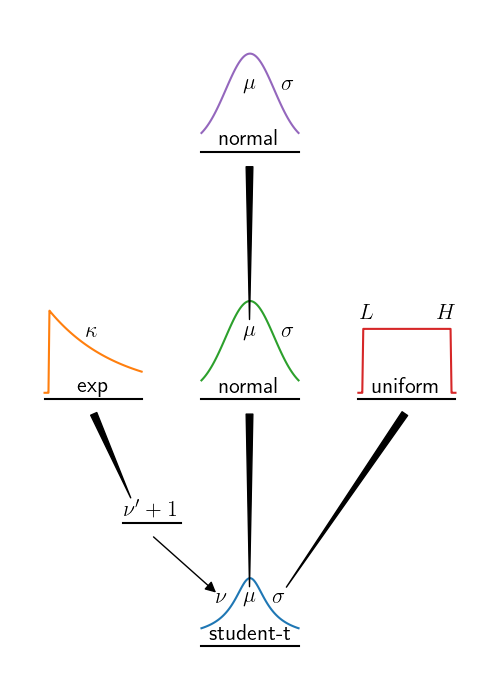
\includegraphics[width=\textwidth]{img/progress-hierarchical}
\end{columns}
\end{frame}

\begin{frame}
\frametitle{Recap of where we are (in pictures!)}
\begin{columns}
\column{.5\textwidth}
Now:
\begin{align*}
\textrm{model: } y      &\sim \operatorname{pdf}(\theta) \\
\textrm{prior: } \theta &= \beta_0 + \beta_1 x \\
                   \beta_0 &\sim \operatorname{pdf}(\varphi_0) \\
                   \beta_1 &\sim \operatorname{pdf}(\varphi_1) \\
                   \varphi_0 &= \Phi_0 \\
                   \varphi_1 &= \Phi_1
\end{align*}
\column{.5\textwidth}
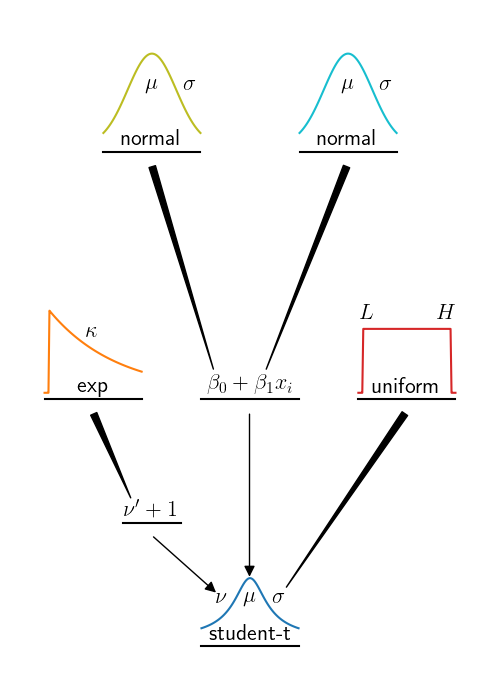
\includegraphics[width=\textwidth]{img/progress-regression}
\end{columns}
\end{frame}







\begin{frame}
\frametitle{Simple Linear Regression}
\begin{columns}
\column{.5\textwidth}
\textbf{Model:} $y = \beta_0 + \beta_1 x + \varepsilon$

\vspace{1em}
\textbf{Note:} Given a particular distribution $x \sim p(X=x)$ the distribution for $y$ will be a smeared version of this (in this case).

\vspace{1em}
\textbf{Homogeneity of variance:} Noise magnitude is independent on scale of input. (Note: Measurement imprecision often increases with scale.)

\vspace{1em}
\textcolor{gray}{\textbf{Homogeneity:} From \emph{homogeneous} + suffix \emph{-ity}}

\column{.5\textwidth}
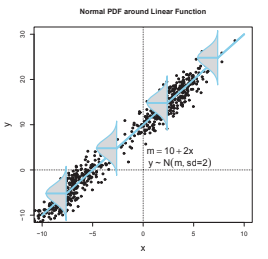
\includegraphics[width=\textwidth]{img/fig17_1}
\end{columns}
\end{frame}



\begin{frame}
\frametitle{Robust Linear Regression (I)}
\begin{columns}
\column{.5\textwidth}
We can often rely on noise being approx. normal. However, specific processes (e.g. transcription errors) can significantly increase probability of outliers.

\vspace{1em}
For Bayesian we can (easily) use other distributions. E.g. Student's t-distribution with heavy tails to resist outliers (w.r.t. the normal distribution).
\column{.5\textwidth}
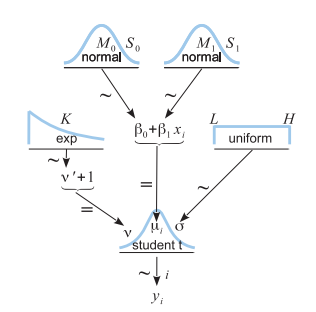
\includegraphics[width=\textwidth]{img/fig17_2}
\end{columns}
\end{frame}

\begin{frame}
\frametitle{Standardisation (I)}
\begin{columns}
\column{.5\textwidth}
Use \emph{standardisation} to massasge data to better fit MCMC generators. Normalises data to be zero-centered and have unit variance. \textcolor{gray}(Weak version of decorrelation, but computationally friendly?)

\vspace{1em} Standardisation can be defined for linear, quadratic, etc. trends.

\vspace{1em} \textbf{Note:} Use only traning data to define your transformation (and inverse).
\column{.5\textwidth}
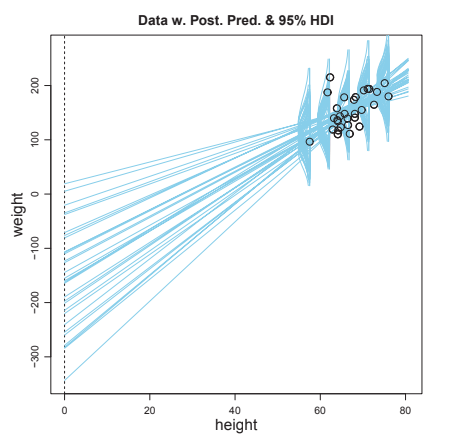
\includegraphics[width=\textwidth]{img/fig17_3_1}
\end{columns}
\end{frame}


\begin{frame}
\frametitle{Standardisation (II)}
\begin{columns}
\column{.5\textwidth}
When using standardised data there is less correlation between slope and offset. (Shown here by the crop.)

\vspace{1em} Additionally, more data moves the estimation farther from the prior. (Not shown: normality paramter smaller for this case, i.e. less normal.)
\column{.5\textwidth}
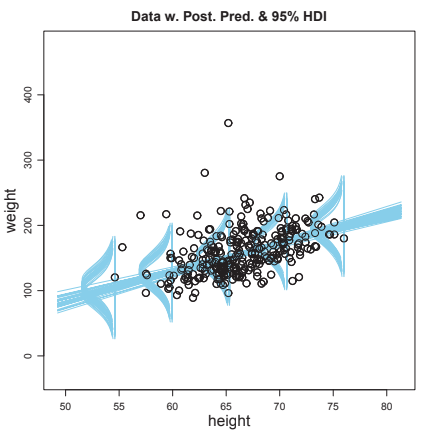
\includegraphics[width=\textwidth]{img/fig17_4_1}
\end{columns}
\end{frame}


\begin{frame}
\frametitle{Structured Noise (I)}
\begin{columns}
\column{.5\textwidth}
Old model
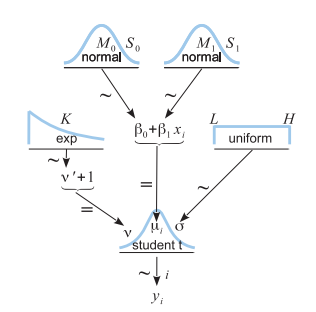
\includegraphics[width=\textwidth]{img/fig17_2}
\column{.5\textwidth}
New model
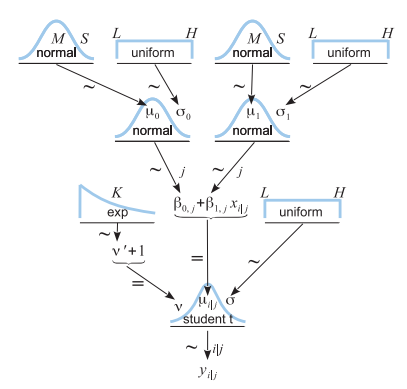
\includegraphics[width=\textwidth]{img/fig17_6}
\end{columns}
\end{frame}

\begin{frame}
\frametitle{Structured Noise (II)}
\begin{columns}
\column{.5\textwidth}
Providing an hierarchical model can significantly change the modelling.

\vspace{1em}
\textbf{Example:} Without grouping, no trend can be seen.
Grouping by individual makes clear that there is significant trend.

\vspace{1em}
\textbf{Note:} Two individuals have only a single sample. Despite this, they have different predictions (the data point pull from group mean).
\column{.5\textwidth}
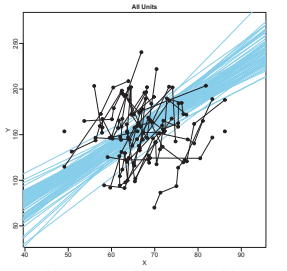
\includegraphics[width=\textwidth]{img/fig17_5_1}
\end{columns}
\end{frame}


\begin{frame}
\frametitle{Extensions etc.}
If there is significant mismodelling (check with posterior predicitve distribution), one can extend the model (also applies for initial modelling).

\vspace{1em}
\textbf{Consider:} 
\begin{itemize}
  \item Trends: linear, quadratic, sinusodial, etc.
  \item Hierarchical models.
  \item Per-individual parameters (req. more data)
  \item Robust distributions (t-distribution in higher level paramters).
  \item Weighting of data (book exemplifies weighting of data credibility).
\end{itemize}

\textbf{Note:} Careful with extending to more paramters, this expands paramter space and can result in less precise estimations.
\end{frame}



\begin{frame}
\frametitle{Recap of where we are}

\textbf{So far:} Modelled a central tendency with added noise.
\begin{align*}
y = \beta_0 + \varepsilon
  \implies y &\sim \mathcal{N}(\beta_0 + \mu_\varepsilon, \sigma_\varepsilon) \\
             &\sim \mathcal{N}(\mu, \sigma)
\end{align*}

\vspace{1em}
\textbf{Now:} Expand structure in central tendency estimation
\begin{align*}
y  = \beta_0 + \beta_1 x + \varepsilon
  \implies y &\sim \mathcal{N}(\beta_0 + \beta_1 x + \mu_\varepsilon, \sigma_\varepsilon)\\
             &\sim \mathcal{N}(\mu=c_0 + \beta_1 x, \sigma)
\end{align*}

\vspace{1em}
\textbf{Improve model:} Posterior predictive check. Model: trends, group-level parameters,  robust distributions, weight data.

\end{frame}






\begin{frame}
\begin{center}
{\huge{Chapter 17}}
\Large
\\\vspace{2em}
End\\
\vspace{1em}
\textcolor{gray}{Appendix below}
\vspace{5em}
\end{center}
\end{frame}








\begin{frame}
\frametitle{Aside: Why assume all noise lies in $y$?}
\textbf{Note:} We assume all measurement noise lies in $y$. Possible since perfect meas. of $y$ and imperfect meas. in $x$ can be interpreted as the inverse (under additive normal noise atleast). Below shown for $x = y + \varepsilon$.

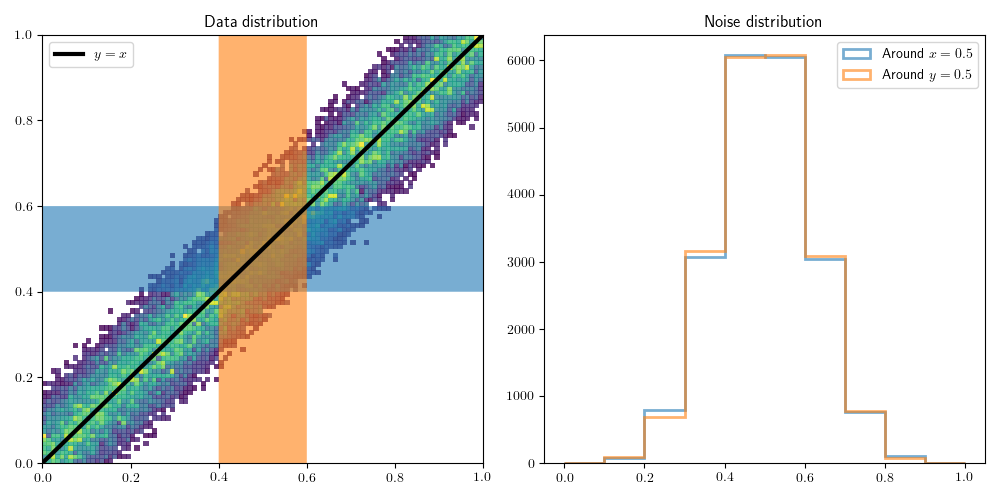
\includegraphics[width=\textwidth]{img/noise}
\end{frame}






\begin{frame}
\frametitle{Aside: Link function}
\textbf{Note:} Incomplete discussion.

\textbf{Suppose} $y\sim\mathcal{N}(\mu, \sigma)$\textbf{:} Modelling the pdf is non-polynomial.

\textbf{Idea:} We can apply a transformation to $y$ to simplify regression. Introduce \emph{link function}:
\begin{align*}
f(y) = v      &= \operatorname{lin}_\beta(x) \\
y = f^{-1}(v) &= f^{-1}(\operatorname{lin}_\beta(x))
\end{align*}

If $v$ is approximately polynomial regression will be simplified, e.g. apply non-linear least squares.

For logistic inverse link function $f^{-1}$ the link function $f$ becomes:
\begin{align*}
f^{-1}(v) &= \operatorname{logistic}(v) \\
f(y)      &= \log \frac{y}{1 - y}
\end{align*}
\end{frame}

\begin{frame}
\frametitle{Aside: Link function}

If one considers $\nu$ as the variable to do regression on, it makes sense that $f$ is the ``primary'' direction.
\begin{align*}
x \overset{\operatorname{lin}}\rightarrow \nu \overset{f^{-1}}\rightarrow y \\
x \overset{\operatorname{lin}^{-1}}\leftarrow \nu \overset{\ f}\leftarrow y 
\end{align*}
\end{frame}

\begin{frame}
\frametitle{Aside: Link function}
Worked example for normal $y$ and $f^{-1}$ logistic:
\vspace{-1em}
\begin{align*}
f(y) &= c_0 \exp - \frac{(x - \mu)^2}{2\sigma^2} \\
     &= \log\left(\frac{c_0 \exp - \frac{(x - \mu)^2}{2\sigma^2}}{1-c_0 \exp - \frac{(x - \mu)^2}{2\sigma^2}}\right) \\
     &= \log\left(c_0 \exp - \frac{(x - \mu)^2}{2\sigma^2}\right) -
        \log\left(1-c_0 \exp - \frac{(x - \mu)^2}{2\sigma^2}\right)\\
     &\approx \log\left(c_0 \exp - \frac{(x - \mu)^2}{2\sigma^2}\right)\\
     &\approx c_1 - \frac{(x - \mu)^2}{2\sigma^2}
\end{align*}
The key in the approximation is that $c_0 \exp - \frac{(x - \mu)^2}{2\sigma^2}$ has a range of $(0, c_0)$ which is $\mathcal{O}(1)$ for reasonable choices of $\sigma$.
\end{frame}

\begin{frame}
\frametitle{Aside: Link function}
\vspace{-1em}
Worked example shown visually (and qualitatively), regression by hand:

\vspace{1em}
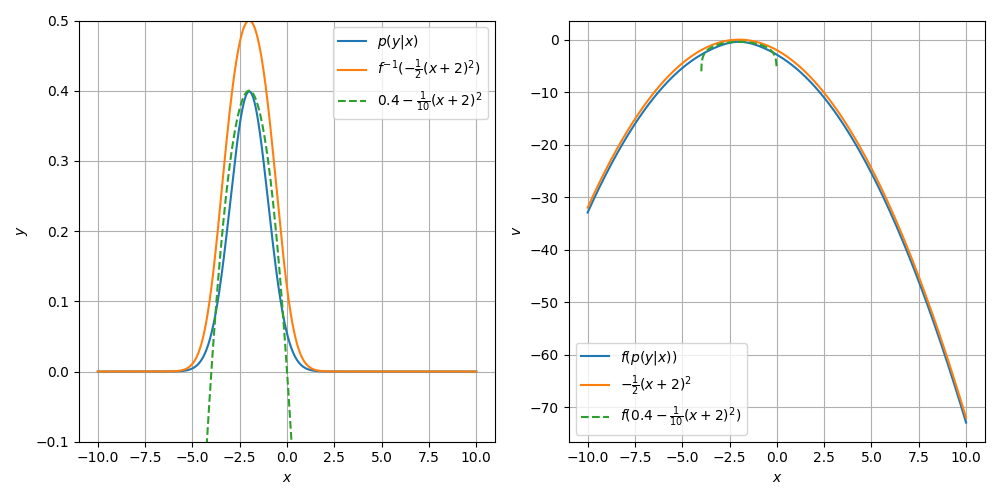
\includegraphics[width=\textwidth]{img/link}
\end{frame}






\end{document} 